\documentclass[journal]{IEEEtran}

\usepackage{graphicx}
\usepackage{diagbox}
\usepackage{changepage}
\newcommand{\var}{\textit}
\newcommand{\proc}{\textbf}
\newcommand{\prop}{\texttt}
\newcommand{\plusplus}{{+}{+}}% Other options: 
\newcommand*\ita[1]{\textit{#1}}
\usepackage{array, booktabs, makecell, multirow}% new
\usepackage{textcomp}
\usepackage[dvipsnames,  x11names, table]{} % add more colors
\usepackage{tikz} % for the cup sketch
% \usepackage{ctable}% http://ctan.org/pkg/ctable
\usepackage{lettrine} % big letter in Intro

\usepackage{siunitx}
\sisetup{per=slash, load=abbr}
\usepackage{tikz}
\usepackage{pgfplots}
\pgfplotsset{width=7cm,compat=1.3}
\pgfplotsset{compat=1.12}
\usepgfplotslibrary{fillbetween} 
\usepgflibrary{shadings}
\usetikzlibrary{backgrounds}
\usetikzlibrary{fit,shapes.geometric}% <--- added

\definecolor{Gray}{gray}{0.9}
\definecolor{Green}{rgb}{0.0, 0.5, 0.0}
\definecolor{Yellow}{rgb}{0.85, 0.65, 0.13}
\definecolor{Grey}{rgb}{0.7, 0.7, 0.7}


% *** GRAPHICS RELATED PACKAGES ***
%
\ifCLASSINFOpdf
  % \usepackage[pdftex]{graphicx}
  % declare the path(s) where your graphic files are
  % \graphicspath{{../pdf/}{../jpeg/}}
  % and their extensions so you won't have to specify these with
  % every instance of \includegraphics
  % \DeclareGraphicsExtensions{.pdf,.jpeg,.png}
\else
  % or other class option (dvipsone, dvipdf, if not using dvips). graphicx
  % will default to the driver specified in the system graphics.cfg if no
  % driver is specified.
  % \usepackage[dvips]{graphicx}
  % declare the path(s) where your graphic files are
  % \graphicspath{{../eps/}}
  % and their extensions so you won't have to specify these with
  % every instance of \includegraphics
  % \DeclareGraphicsExtensions{.eps}
\fi

\begin{document}
%

\title{Detection of Object Properties from Human-Human Handover Actions and Applications in Robotics}
%
\author{Nuno Ferreira Duarte$^{1,2}$, 
        Aude Billard$^2$, and 
        Jos\'{e} Santos-Victor$^{1}$ 
        
\thanks{Corresponding author: Nuno Ferreira Duarte.}
\thanks{This work was partially supported by the RBCog-Lab research infrastructure, Funda\c{c}\~{a}o para a Ci\^{e}ncia e a Tecnologia (FCT) with reference UID/EEA/50009/2019, and the PhD grant with reference PD/BD/135116/2017 of Nuno Ferreira Duarte.}
\thanks{$^{1}$Vislab, Institute for Systems and Robotics, Instituto Superior T\'{e}cnico, Universidade de Lisboa, Portugal.
{\tt\{nferreiraduarte, jasv\}@isr.tecnico.ulisboa.pt}}

\thanks{$^2$LASA, Swiss Federal Institute of Technology, Lausanne, Switzerland. {\tt \{nuno.ferreiraduarte, aude.billard\}@epfl.ch.}}
}

% The paper headers
\markboth{IEEE ROBOTICS AND AUTOMATION LETTERS, ~Vol.~?, No.~?, Apri~2021}%
{Shell \MakeLowercase{\textit{et al.}}: Bare Demo of IEEEtran.cls for IEEE Journals}
% The only time the second header will appear is for the odd numbered pages
% after the title page when using the twoside option.
% 
% *** Note that you probably will NOT want to include the author's ***
% *** name in the headers of peer review papers.                   ***
% You can use \ifCLASSOPTIONpeerreview for conditional compilation here if
% you desire.

% If you want to put a publisher's ID mark on the page you can do it like
% this:
%\IEEEpubid{0000--0000/00\$00.00~\copyright~2015 IEEE}
% Remember, if you use this you must call \IEEEpubidadjcol in the second
% column for its text to clear the IEEEpubid mark.


% make the title area
\maketitle

\begin{abstract}

% witty, interesting take on robotics, and human interactions
Human interaction involves very sophisticated non-verbal communication skills like understanding the goals and actions of others and coordinating 

% contributions 
analyse the kinematic motion of the human arm during handovers of cups and glasses under two conditions: (i) empty, and (ii) filled with water. From the kinematic motion, it was recognized two distinct strategies according to the human perceived challenge: (i) unrestricted, free motion - natural manipulation; and (ii) constrained, challenging motion due to danger of spilling - careful manipulation. Secondly, we compare two computational model approaches that aim to describe the two kinematic strategies observed. Thirdly, from the approach with the best results, we embedded the model in a robot controller with a human-in-the-loop where the approach is tested on human-object interaction and human-robot interaction scenarios. 
The results show that the best approach can generalize well to unknown people, cups, and new human handover scenarios (datasets). The robot controller proves that it can be applied to multiple human-robot tasks and provide accurate information on the object properties or human motion preference. 

% results


\end{abstract}

% Note that keywords are not normally used for peerreview papers.
% \begin{IEEEkeywords}
% IEEE, IEEEtran, journal, \LaTeX, paper, template.
% \end{IEEEkeywords}

%%%%%%%%%%%%%%%%%%%%%%%%%%%
\section{Introduction}

\lettrine{C}{ontainers} such as the ones that carry liquids, like cups, glasses, mugs, produce a response on the human when transporting depending on the fillness level. Mayer et al. \cite{mayer_walking_2012} provides an example of a highly familiar challenge to anyone in academia, walking back to one's office while taking mug filled with coffee. They've found that humans try to solve the issue of spilling by either estimating the frequency of sloshing of the liquid and counteract the resonance to suppress it, or by simply being pro-active and careful during manipulation. The authors justify the reason for picking one of the approach down to individual preference, however we argue that most would resort to the latter option as is the one that requires the least effort and with less accidents. As such, this paper aims at providing an in depth scope of the manipulation strategies for cups filled with water or completely empty. As it provides two opposite scenarios with contrasting levels of difficulty. The purpose of this analysis is so that it can provide useful features that robots can take advantage. In a factory plant, robots can understand inherent properties of objects, such as fragility or breakableness, by observing how humans interact with it, or in an elderly home, where a robot caretaker needs to adapt to the motor capabilities of each individual. 

% the challenge, the different ways that people have tried to use to solve it

% soa
% you focus on the work related, the neuroscience behind it, the psychology behind it, the non-verbal communication behind it, the different manipulation works, the different handover approaches, the affordances of objects, the impact that weight and object properties has on the human manipulation, mention your previous work

% neuroscience
\cite{alaerts_force_2010} Observing lifting objects of different weights modulate M1, primary motor cortex, in a muscle-specific way. Cortical representation areas in M1 that control the specific muscles used in the observed lifting actions became increasingly facilitated. The higher the M1 excitability is, the heavier is the object. It may contribute, at least partly, to the observer's ability to infer the weight of the object. 
 \cite{senot_effect_2011}
Explicit weight-related information => written labels on the objects. - and if there is a conflict between label and object weight. 
Discussion: Hidden (object hidden-only kinematic cues) - significant modulation of MEPs amplitude according with the force required to hold the object. Visible (visible object and kinematic cues) - not significant different. Labels (labels on the object) - influence the observers - same label for light and heavy object then MEPs amplitude was not significantly different. - different labels => same as in Hidden or Visible conditions. 
Previous results: high-level semantic cues, such as labels, may influence low-level motor behaviour during execution. - Any time a conflict is present between explicit and implicit movement-related information, the observers motor system stops its mirroring of the observed action -> mirror mechanisms is not blind to semantic info. - predominance of kinematic cues over intrinsic object properties in coding force required to execute an observed lifting action. 
\cite{lindemann_grasping_2011} biological grasping actions modulated the observer's attention whereas the perception of inanimate stimuli does not.

the psychology -
\cite{jamone_affordances_2018} A very important paper from JSV to reference
 \cite{sciutti_development_2019}
Infer the weight of unknown object - intrinsic feature not directly accessible through vision. Judge weight of objects after watching videos of an actor lifting. At age 6 they can estimate difference in weight by observing different videos of objects. At age 10 the variability of estimation decreases and the accuracy increases. However they usually underestimate the weight. Adults are better at estimating. Improvement of performance reflects the development of children's motor control. - Children's stature was more reliable than their chronological age -> Body heights more directly related to growth than age. - Features important to estimate weight? Temporal and spatial-temporal features of the movements. => duration and absolute velocity. 
 \cite{sciutti_understanding_2014}
By action observation we can infer the goal of the action or even the object's weight. This implicit understanding is developed early in childhood and is supposedly based on a common motor repertoire between the cooperators. Results: subjects can reach a performance in weight recognition from robot observation comparable to that obtained during human observations with no need of training. 3 experiments are made in this paper - neural (doing nothing), human action/movie watching - active (while object lifting), robot action - neutral. Known (know the weight and grasp before), Human condition (unknown weight), Interaction (not grasping before). 
Discussion: robot lifting with standard motion => humans can not estimate weight => obviously! Robot proportional allows! -> weight reading derives a generalization of the skills normally adopted in HHI. Human explicit kinematic whether it is a human or a robot. -> However the robot must exhibit familiar motor behaviours to the human. Otherwise it could cause detrimental effects => uncanny valley. How strong is the human influences how we estimate the object. 

the non-verbal cues -
\cite{mavridis_review_2015} apparently this is a review on non-verbal cues (I havent read it)
\cite{duarte_action_2018} my paper "Work from me points that human non-verbal cues from eyes, head, and arm movements decode action intention, and when incorporating onto a robot, it provides similar information to read the robot's intention."
\cite{palinko_communicative_2015} passing an object relies on the non-verbal communication associated to the passer's motion. Ask the human's to judge the weight of the object
\cite{sciutti_humanizing_2018} elaborating several important design factors. we are conviced that they build a solid basis and an effective strategy for the development of humane robots. "the ability of the robot to anticipate human behaviour required a very deep knowledge of the motor and cognitive bases of human-human interaction
\cite{admoni_robot_2016} 

manipulation:
\cite{hamilton_kinematic_2007} perceptual weight judgment provides a powerful method to study our interpretation of other people's actions, but it is not known what sources of information are used in judging weight
\cite{kjellstrom_visual_2011} learning the affordance of objects from human demonstration (what else?)
\cite{santina_learning_2019} LfD

handovers - 
\cite{Medina2016} only focused on the handover, not the manipulation/transportation. The robot waits for the load share to pass a certain, hand-tuned, human based, threshold.

careful - 
previous paper \cite{duarte_human_2020} This paper is the prequel to this work.
\cite{lastrico_careful_2021} the most recent paper that finally measures carefulness. I NEED TO READ THIS PAPER

% structure of the paper
We start by defining the human-human interaction scenario detailed in Section \ref{sec:human}, describing the experiments, the sensor information collected, and the data chosen to analyse the handover of cups. The human non-verbal cues extracted from the HHI dataset are employed on computational models of kinematic approaches of handover of empty and full of water cups (Section \ref{sec:model}). Two computational models are mentioned, one novel and one previously proposed, that from the handover trajectories extract features to express the kinematic strategies of manipulating empty and full of water cups. The presented classifier allows for a fair metric of both models performance. The accuracy of each model is measured on how well it can distinguish handovers of empty cups as natural manipulations (not careful), and handover of water filled cups as a careful manipulation. In Section \ref{sec:results} it presents additional classification results in order to understand the impact of different types of cups, as well as, other datasets of human handovers with unknown cups, and unknown participants. The developed computational model with the best classification accuracy is incorporated in a robotic controller in Section \ref{sec:robot}. The model runs in a human-in-the-loop system which provides the robot with information on the cup or object interacted by the human as to adapt its motor control approach when grasping or manipulating. The Section \ref{sec:conc} we discuss the findings from our analysis of the human-human data, classification accuracy of the computational models, and human-robot experiments, and finish by outlining future work proposals.  


\section{Human to Human Handover}
\label{sec:human}

In this section we describe the human-human experiments performed, the different objects, and the acquired data for analysis of handover motions. The section includes analysis of the handover motion in terms of velocity over the trajectory as well as velocity along time, followed by an overall discussion on the different types of handover motions. 

\subsection{Experimental Scenario}

The HHI dataset was gathered as a collaboration between 
École polytechnique fédérale de Lausanne (EPFL) and Karlsruher Institut für Technologie (KIT) \cite{starke_force_2019}. It involves two humans interacting with an object whether to grasp and handover to one another, or to manipulate and place it on a table. The focus of this work is solely on the handover motion. Figure \ref{fig:epfl_dataset} shows a frame of the handover trajectory of the different cups for each of the participants. The experiments includes data of 4 participants, all male, age between 25-35 years old, with a graduate academic background. The recorded data includes motion tracking markers from the OptiTrack system on the participant's wrist and on the cups, as well as data gloves from the CyberGlove system on the participant's hand (not used in this work).

    \begin{figure}
        \centering
        \begin{tabular}{@{}c@{}}
            \centering
            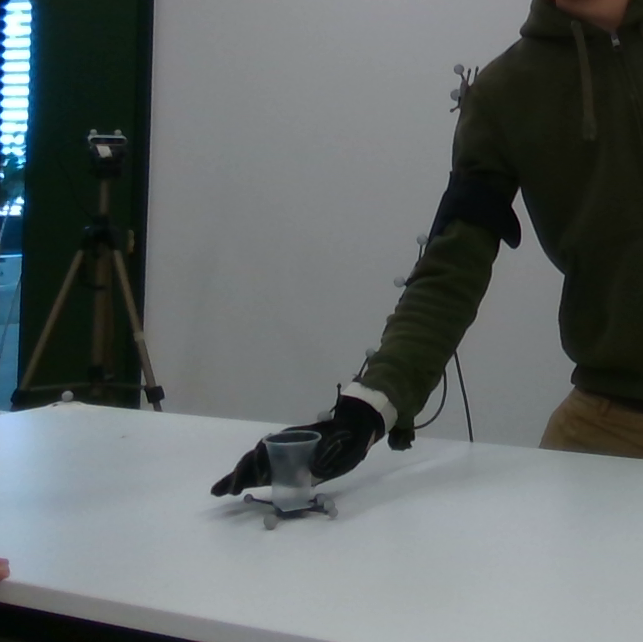
\includegraphics[width=0.225\textwidth,height=0.15\textheight]{Images/frame000023.png}
        \end{tabular}
        \begin{tabular}{@{}c@{}}
            \centering 
            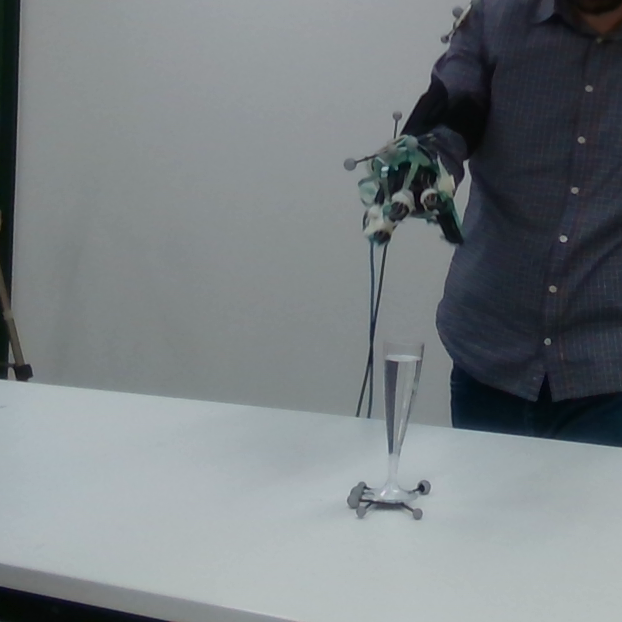
\includegraphics[width=0.225\textwidth,height=0.15\textheight]{Images/frame000046.png}
        \end{tabular}
        \baselineskip
        \begin{tabular}{@{}c@{}}
            \centering 
            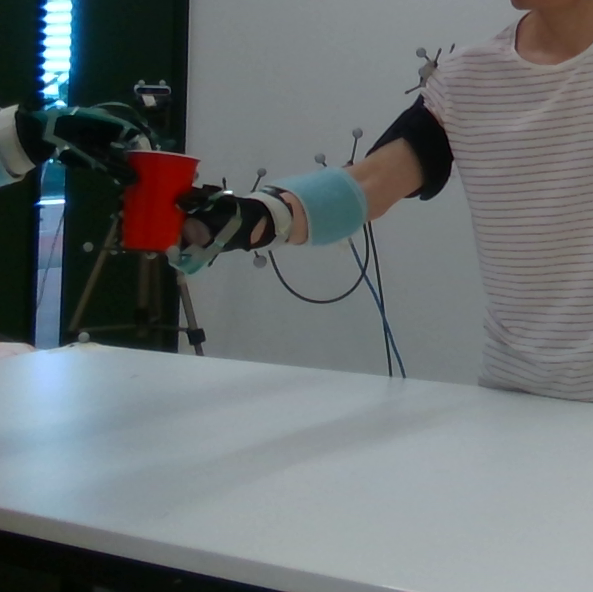
\includegraphics[width=0.225\textwidth,height=0.15\textheight]{Images/frame000117.png}
        \end{tabular}
        \begin{tabular}{@{}c@{}}
            \centering 
            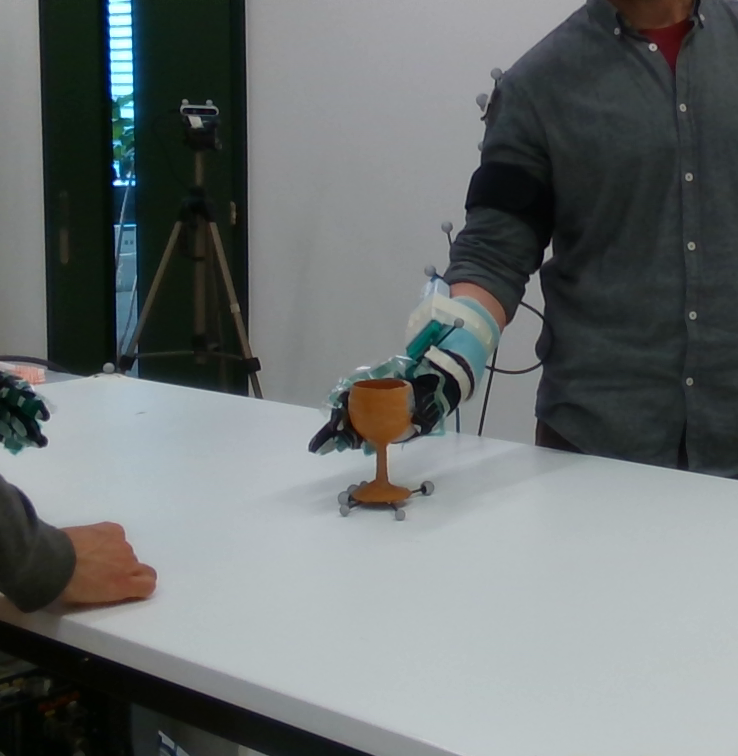
\includegraphics[width=0.225\textwidth,height=0.15\textheight]{Images/frame000144.png}
        \end{tabular}
        \caption{The 4 participants with the 4 cups}
        \label{fig:epfl_dataset}
    \end{figure}
    
The handovers of the cups happen under two distinct situations: (i) an empty cup, and (ii) a cup 90\% filled with water. Each participant hands-over the different cups to a second participant (also present in the dataset but not analysed during the handover), and each cup is manipulated for both conditions. The cups relevant for this work are the red plastic cup (bottom-left), the transparent plastic cup (top-left), the champagne plastic cup (top-right), and the opaque wine glass (bottom-right). The handover trajectory is recorded at 120 Hz, taking on average 1-3 seconds, corresponding to 100-300 data points. A total of 100 handover trajectories are segmented for all the participants with the 4 cups in the two conditions.

The purpose of performing these experiments has to do with the lack of available datasets on human manipulating cups with different internal properties, such as material composition, shape, weight, and with varying conditions such as liquid level. There is also not been, to our knowledge, an extensive analysis on the impact of those varying properties on the kinematic control approaches of humans and possible applications to robots. 

\subsection{Handover Motion Analysis}

The handover motions are 3D Cartesian coordinates over time which begin at the moment of pickup (grasp) and finish when the cup is safely held by the other participant (handover). During the HHI experiments the participant could grasp the cup irrespective of the hand configuration and the handover location could be in whatever 3D space bounded by the table separating the two interactants. This gave rise to several different grasp configurations and a disparity on the duration/length of the handover trajectories. Bear in mind that it was not possible to re-grasp the cup or change grasp configuration during the handover, and the cup would have to start upwards on the table for every interaction. 

    \begin{figure}
        \centering
        \begin{tabular}{@{}c@{}}
            \centering
            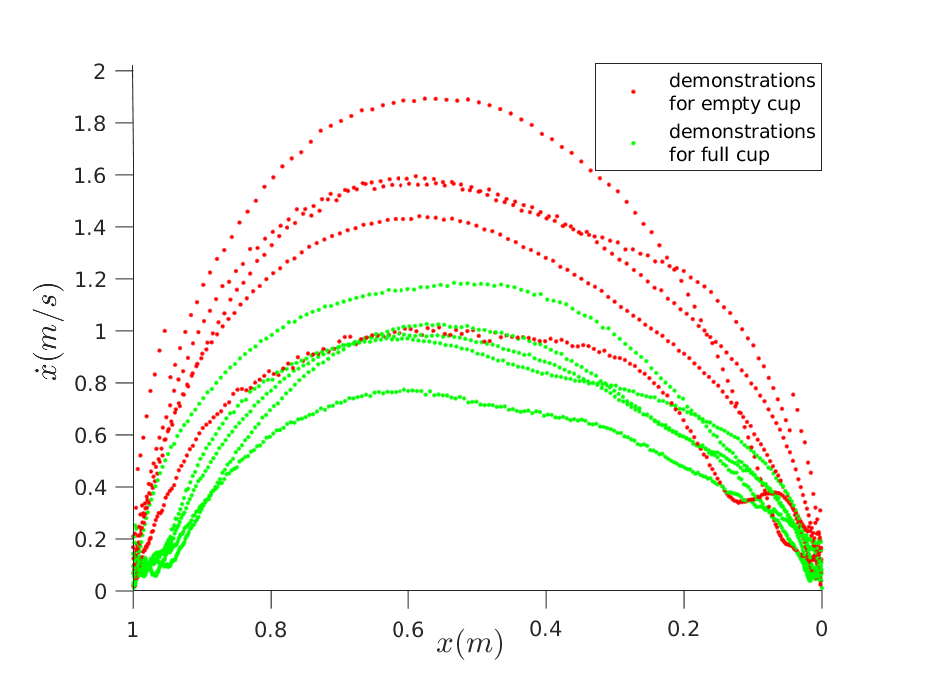
\includegraphics[width=0.48\textwidth,height=0.25\textheight]{Images/vel_distance_plot.eps}
        \end{tabular}
        \baselineskip
        \begin{tabular}{@{}c@{}}
            \centering 
            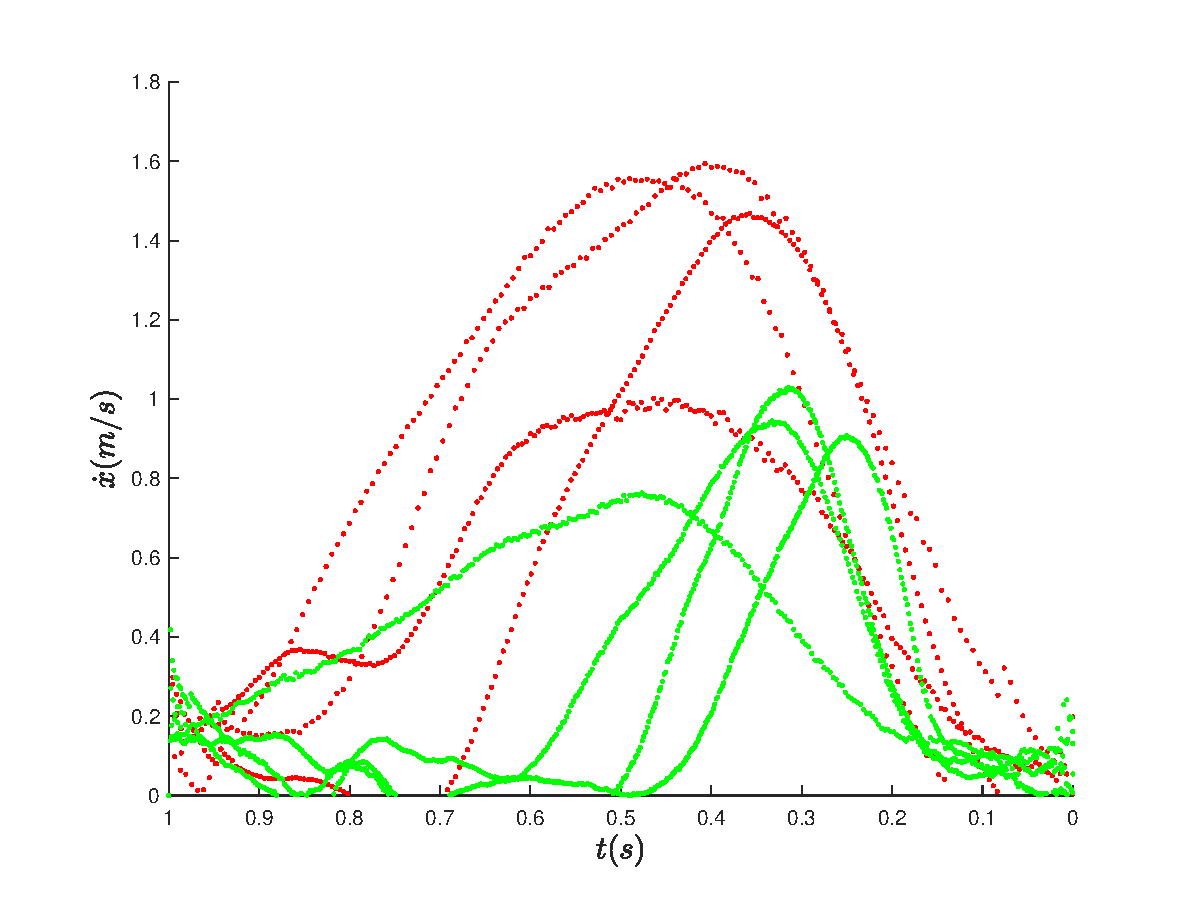
\includegraphics[width=0.48\textwidth,height=0.25\textheight]{Images/vel_time_plot.eps}
        \end{tabular}
        \caption{Sample of the dataset. Velocity/distance (top) and velocity/time (bottom).}
        \label{fig:vel_distance_time}
    \end{figure}

To capture the kinematic of the wrist for all the trials of every participant, cup, and cup condition, irrespective of the starting location in the grasp and the final position for the handover, it was decided to apply min-max normalization before reducing the dimensionality to 1-D vector by calculating the euclidean norm of the $x, y,$ and $z$ dimensions. This re-scales the data to the range [0, 1] where 0 is the final step, refer to as the handover, and 1 is the initial step, refer to as the grasp of the cup from the table. Figure \ref{fig:vel_distance_time} depicts handover trajectories, after post-processing, with respect to the first derivative of the euclidean norm. The plot on the top exhibits the kinematic evolution of the human wrist with respect to the position in the handover trajectory. The bottom plots exhibits the same dataset sample of demonstrations and it represents the velocity of the human wrist with respect to time during the handover trajectory. The purpose of these representations is to identify the acceleration and deceleration phase which is of relevance to the approaches presented in the next section. 

\subsection{Discussion}

The common trait of all demonstrations is the typical bell-shape for the velocity profile as humans choose a minimum jerk approach for the hand trajectory. This has been identified in previous works in point-to-point human motion \cite{flash} and this behaviour manifests, likewise, in human object handovers. In contrast, the most notable difference is on the bell-shape's peak, i.e. the maximum velocity reached by the human. As seen in the demonstrations, the difference can be noticed when distinguishing the cups by the level of water contents, as most of the handovers of empty cups reached higher maximum velocities as the handovers of the same cup full of water. The reason is straightforward as a cup filled with water presents an additional challenge during manipulation: transporting the contents inside without spilling or breaking. There is also the added weight of the liquid to the overall mass of the cup, however we argue that the effect of a liquid moving inside a cup due to the oscillations of the human manipulation is more impactfull in deterring quick and jerky movements than a particular heavy object. Additionally, humans tend to build preconceptions of their surroundings and before manipulation tend to estimate the object's mass and the required force to lift and manipulate. As a result, a novel object with an unexpected heavy mass might invoke a slower manipulation in the first encounter but after some attempts, the human adapts the motor control approach and the manipulation can be more natural. This familiarity procedure is not present when manipulating cups with liquid inside, as the content is visible from the first encounter but the risk of spilling is constantly present. For this reason, we consider the level of water to be the most important factor. In Section \ref{sec:results} we will discuss in depth the different cups and the impact of water contents. 

In this section we proceeded to present the human-human experiments performed and the data recorded. From the dataset, the handover trajectories were segmented, post-processed to extract the acceleration and deceleration phase of the wrist movement for any handover of empty or full water cups. From the analysis it was detected that manipulating cups full of water would usually originate in a slower, less abrupt motion, compared to empty cups. In the next section the processed handover segmentations will be used to learn models for detecting different manipulation behaviours.


\section{Modelling of Handover Manipulations}
\label{sec:model}
%intro
In this Section we present the approaches that model human manipulation of cups in two situations: (i) empty cup, or (ii) water level at around 90 \%. From the discussion in Section \ref{sec:human} and the sample data illustrated in Figure \ref{fig:vel_distance} we can argue that there are two possibilities for modelling the human manipulation in the handover context: (i) the acceleration phase, and (ii) the deceleration phase. The acceleration phase represents the interval where the object begins at rest position, as the human grasp the object, and is proceeded by an increase in velocity of the cup during the human manipulation. Whilst the deceleration phase indicates the approach stage to handover the cup to another person, indicated by a gradual decrease in velocity until a stationary state is reached for the handover be completed.
To note that this behaviour is also present for a pick-and-place action \cite{flash_models_2013} where the human, instead of handing over, places safely the cup in a new location, resulting in decrease velocity of the cup for a safe and steady placement.  

The deceleration phase was first implemented in the previous paper \cite{duarte_human_2020} and it provided a direct comparison of velocities for the two cases situations. This was possible as the extraction of the deceleration phase during the cup manipulation revealed the maximum velocities and its evolution towards the rest stage, i.e. handover completion. From this approach we model the velocity as a function of the distance towards the handover for both situations. 

- now move to the section

- don' forget to present the second approach

% add a small introduction of the reason for two approaches

\begin{figure}[h]
\tikzset{every picture/.style={line width=0.75pt}} %set default line width to 0.75pt    
\begin{tikzpicture}[x=0.75pt,y=0.75pt,yscale=-1,xscale=1]
%uncomment if require: \path (0,394); %set diagram left start at 0, and has height of 394

%Shape: Rectangle [id:dp8171705286563367] 
\draw   (0.5,192.38) -- (48.57,192.38) -- (48.57,219.61) -- (0.5,219.61) -- cycle ;
%Shape: Rectangle [id:dp16137444864977923] 
\draw   (95.51,2.5) -- (224.25,2.5) -- (224.25,20.16) -- (95.51,20.16) -- cycle ;
%Shape: Rectangle [id:dp6063905810492368] 
\draw  [dash pattern={on 4.5pt off 4.5pt}] (62.63,39.3) -- (250.83,39.3) -- (250.83,161) -- (62.63,161) -- cycle ;
%Image [id:dp43598404181394723] 
\draw (156.73,100.15) node  {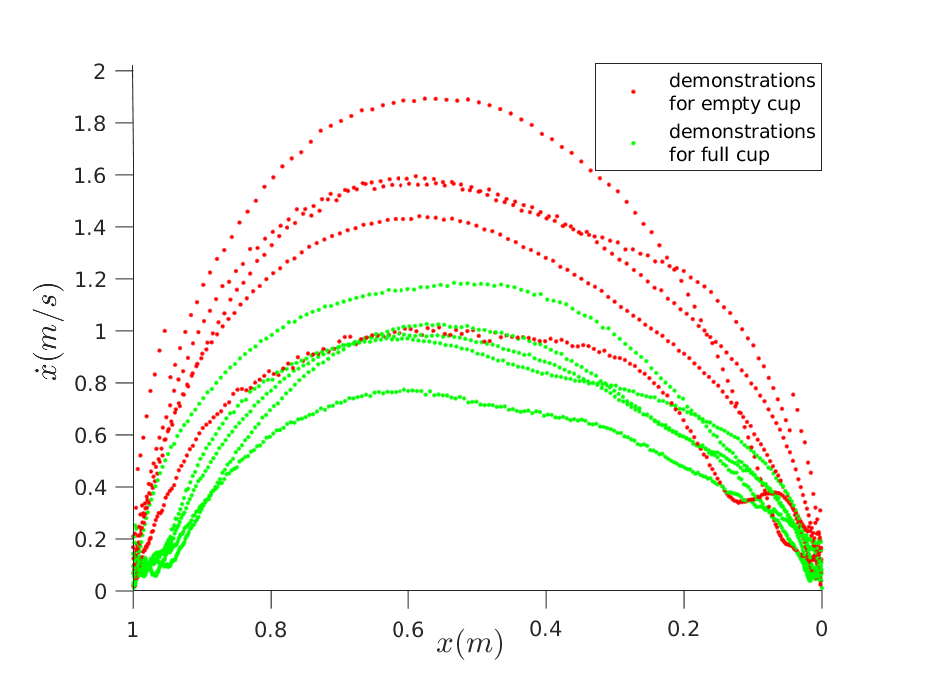
\includegraphics[width=141.15pt,height=91.28pt]{Images/vel_distance_plot.eps}};
%Shape: Rectangle [id:dp7136803259697821] 
\draw  [color={rgb, 255:red, 255; green, 255; blue, 255 }  ,draw opacity=0 ][fill={rgb, 255:red, 245; green, 166; blue, 35 }  ,fill opacity=0.55 ] (156.73,39.3) -- (250.83,39.3) -- (250.83,161) -- (156.73,161) -- cycle ;
%Shape: Rectangle [id:dp4989299581398505] 
\draw  [color={rgb, 255:red, 255; green, 255; blue, 255 }  ,draw opacity=0 ][fill={rgb, 255:red, 75; green, 87; blue, 211 }  ,fill opacity=0.39 ] (62.63,39.3) -- (156.73,39.3) -- (156.73,161) -- (62.63,161) -- cycle ;
%Straight Lines [id:da2860186468382656] 
\draw    (156.82,21.39) -- (156.85,34.49) -- (156.86,35.07) ;
\draw [shift={(156.87,37.07)}, rotate = 269.53] [color={rgb, 255:red, 0; green, 0; blue, 0 }  ][line width=0.75]    (7.65,-3.43) .. controls (4.86,-1.61) and (2.31,-0.47) .. (0,0) .. controls (2.31,0.47) and (4.86,1.61) .. (7.65,3.43)   ;
%Rounded Rect [id:dp6443750059991944] 
\draw   (85.68,191.92) .. controls (85.68,186.88) and (89.77,182.8) .. (94.81,182.8) -- (219.21,182.8) .. controls (224.25,182.8) and (228.34,186.88) .. (228.34,191.92) -- (228.34,219.3) .. controls (228.34,224.34) and (224.25,228.43) .. (219.21,228.43) -- (94.81,228.43) .. controls (89.77,228.43) and (85.68,224.34) .. (85.68,219.3) -- cycle ;
%Rounded Rect [id:dp0531242957100273] 
\draw   (93.69,194.2) .. controls (93.69,190.14) and (96.99,186.84) .. (101.05,186.84) -- (145.23,186.84) .. controls (149.29,186.84) and (152.59,190.14) .. (152.59,194.2) -- (152.59,216.28) .. controls (152.59,220.35) and (149.29,223.64) .. (145.23,223.64) -- (101.05,223.64) .. controls (96.99,223.64) and (93.69,220.35) .. (93.69,216.28) -- cycle ;
%Rounded Rect [id:dp10795879107477857] 
\draw   (163.25,195.31) .. controls (163.25,191.45) and (166.38,188.32) .. (170.24,188.32) -- (215.15,188.32) .. controls (219.01,188.32) and (222.15,191.45) .. (222.15,195.31) -- (222.15,216.28) .. controls (222.15,220.14) and (219.01,223.27) .. (215.15,223.27) -- (170.24,223.27) .. controls (166.38,223.27) and (163.25,220.14) .. (163.25,216.28) -- cycle ;
%Straight Lines [id:da9553234338793252] 
\draw    (52.94,206.85) -- (80.94,206.73) ;
\draw [shift={(80.94,206.73)}, rotate = 180] [color={rgb, 255:red, 0; green, 0; blue, 0 }  ][line width=0.75]    (8.74,-3.92) .. controls (5.56,-1.84) and (2.65,-0.53) .. (0,0) .. controls (2.65,0.53) and (5.56,1.84) .. (8.74,3.92)   ;
%Straight Lines [id:da8975459341516769] 
\draw    (231.22,207.35) -- (248.04,207.6) ;
\draw [shift={(250.04,207.63)}, rotate = 180.85] [color={rgb, 255:red, 0; green, 0; blue, 0 }  ][line width=0.75]    (8.74,-3.92) .. controls (5.56,-1.84) and (2.65,-0.53) .. (0,0) .. controls (2.65,0.53) and (5.56,1.84) .. (8.74,3.92)   ;
%Rounded Rect [id:dp6783697061768484] 
\draw   (254.14,195.79) .. controls (254.14,192.08) and (257.15,189.07) .. (260.86,189.07) -- (301.14,189.07) .. controls (304.85,189.07) and (307.86,192.08) .. (307.86,195.79) -- (307.86,215.95) .. controls (307.86,219.67) and (304.85,222.68) .. (301.14,222.68) -- (260.86,222.68) .. controls (257.15,222.68) and (254.14,219.67) .. (254.14,215.95) -- cycle ;
%Straight Lines [id:da7778502429910122] 
\draw    (309.58,206.76) -- (320.37,206.83) ;
\draw [shift={(322.37,206.84)}, rotate = 180.37] [color={rgb, 255:red, 0; green, 0; blue, 0 }  ][line width=0.75]    (8.74,-3.92) .. controls (5.56,-1.84) and (2.65,-0.53) .. (0,0) .. controls (2.65,0.53) and (5.56,1.84) .. (8.74,3.92)   ;
%Straight Lines [id:da060082135680290416] 
\draw    (155.97,163.81) -- (156,176.9) ;
\draw [shift={(156,178.9)}, rotate = 269.87] [color={rgb, 255:red, 0; green, 0; blue, 0 }  ][line width=0.75]    (8.74,-2.63) .. controls (5.56,-1.12) and (2.65,-0.24) .. (0,0) .. controls (2.65,0.24) and (5.56,1.12) .. (8.74,2.63)   ;
%Straight Lines [id:da8234214050961214] 
\draw    (66.94,206.79) -- (67.37,242.34) ;
%Straight Lines [id:da5201978982400552] 
\draw    (283.93,242.41) -- (283.75,227.01) ;
\draw [shift={(283.72,225.01)}, rotate = 449.31] [color={rgb, 255:red, 0; green, 0; blue, 0 }  ][line width=0.75]    (8.74,-3.92) .. controls (5.56,-1.84) and (2.65,-0.53) .. (0,0) .. controls (2.65,0.53) and (5.56,1.84) .. (8.74,3.92)   ;
%Straight Lines [id:da7606688623528574] 
\draw    (67.37,242.34) -- (283.93,242.41) ;

% Text Node
\draw (239.25,42.92) node [anchor=north west][inner sep=0.75pt]  [font=\scriptsize] [align=left] {1};
% Text Node
\draw (66.3,41.74) node [anchor=north west][inner sep=0.75pt]  [font=\scriptsize,rotate=-359.78] [align=left] {2};
% Text Node
\draw (98.28,192.99) node [anchor=north west][inner sep=0.75pt]  [font=\scriptsize] [align=left] {\begin{minipage}[lt]{34.85pt}\setlength\topsep{0pt}
\begin{center}
Careful \\Behaviour
\end{center}

\end{minipage}};
% Text Node
\draw (165.25,194.44) node [anchor=north west][inner sep=0.75pt]  [font=\scriptsize] [align=left] {\begin{minipage}[lt]{38.82pt}\setlength\topsep{0pt}
Not Careful
\begin{center}
Behaviour
\end{center}

\end{minipage}};
% Text Node
\draw (263.36,193.57) node [anchor=north west][inner sep=0.75pt]  [font=\scriptsize] [align=left] {\begin{minipage}[lt]{26.52pt}\setlength\topsep{0pt}
\begin{center}
Belief \\System
\end{center}

\end{minipage}};
% Text Node
\draw (234.93,190.43) node [anchor=north west][inner sep=0.75pt]  [font=\small]  {$Y$};
% Text Node
\draw (152.65,229.17) node [anchor=north west][inner sep=0.75pt]  [font=\small]  {$\dot{x}$};
% Text Node
\draw (85.38,168.08) node [anchor=north west][inner sep=0.75pt]  [font=\footnotesize] [align=left] {Model};
% Text Node
\draw (254.08,175.6) node [anchor=north west][inner sep=0.75pt]  [font=\footnotesize] [align=left] {Classifier};
% Text Node
\draw (95.32,21.79) node [anchor=north west][inner sep=0.75pt]  [font=\footnotesize] [align=left] {Dataset};
% Text Node
\draw (95.51,5.5) node [anchor=north west][inner sep=0.75pt]  [font=\footnotesize,rotate=-359.96,xslant=0] [align=left] {Human Demonstrations};
% Text Node
\draw (4.9,199.72) node [anchor=north west][inner sep=0.75pt]  [font=\footnotesize] [align=left] {Human};
\
\end{tikzpicture}
  \caption{The Diagram}
  \label{fig:diagram}
\end{figure}


This here Figure \ref{fig:diagram}
Let $x \in D \subset \mathbb{R}^{+}$ denote the distance of the human wrist towards the handover meeting point. 

\subsection{Deceleration Phase}

- present a short version of the deceleration phase (previous paper)

- explain why you decide to resort to this new approach


Consider a behavior encoded as a state-dependent dynamical system (DS)
%
\begin{equation}
\dot{x} = \pmb{\textnormal{f}}(x)
\label{eq:1}
\end{equation}
where $\pmb{\textnormal{f}}:\mathbb{R}^{+} \to \mathbb{R}^{+}$ is a continuous and continuously differentiable function, with a single equilibrium point ${\dot{x}_d}^* = \pmb{\textnormal{f}}(x^*)$. $x^{*}$ is set at the origin and it is globally asymptotic stable such that $\dot{x}^* = \textnormal{f}(x^{*}) = 0$ which is guaranteed under a Lyapunov function $V(x):\mathbb{R}^{+} \rightarrow \mathbb{R}^{+}$.

Our approach defines each ``carefulness'' condition, \textit{careful} and \textit{not careful}, as two distinct DS. Each DS is encoded using Gaussian Mixture Models (GMM) which defines a joint distribution function $\mathcal{P}({{x}^{t}}_n, {\dot{x}^{t}}_n | \Theta) = \sum_{k=1}^{K} \pi^{k} \mathcal{N}({{x}^{t}}_n, {\dot{x}^{t}}_n, \mu^{k}, \Sigma^{k})$ over the data as mixture of $K$ Gaussian distributions \cite{khansari2011learning}, where $\pi^{k}$, $\mu^{k}$, and $\Sigma^{k}$ are, respectively, the prior component, mean, and covariance matrix of the $k$th Gaussian. $x_n^t$ is $n$th trajectory of $x$ at time $t$, and $\dot{x}_n^t$ is its derivative. Fig. \ref{fig:motion} illustrates the position ($x$) and velocity ($\dot{x}$) relations for \textit{careful} and \textit{not careful} motions. To compute the DS from Eq. (\ref{eq:1}) the posterior mean of $\mathcal{P}({\dot{x}^{t}}_n|{{x}^{t}}_n)$ is estimated which approximates it to:
%
\begin{equation}
\hat{\dot{x}} = \sum_{n=1}^{K} h^{k}(x) (\Sigma^{k}_{\dot{x}x}(\Sigma^{k}_{xx})^{-1} (x - \mu^{k}_{x}) + \mu^{k}_{\dot{x}})
\label{eq:2}
\end{equation}
where $h^{k}(x) = \frac{\pi^{k} \mathcal{N}({{x}^{t}}, {\dot{x}^{t}}, \mu^{k}, \Sigma^{k})}{\sum_{i=1}^{K} \pi^{k} \mathcal{N}({{x}^{t}}_n, {\dot{x}^{t}}_n, \mu^{i}, \Sigma^{i})}$, $h^{k}(x) > $ 0, and $\sum_{n=1}^{K} h^{k}(x)$ = 1. The GMMs are computed using the stable estimator of dynamical systems (SEDS) approach \cite{khansari2011learning}. 

- mention limitations of this approach. The model is focused on the latter stage of the manipulation hence the recognition happens later. The models did not provide useful results for regions outside of the learned models. When testing the generated velocities for both models were very similar not allowing the classifier to distinguish between the two. 

\subsection{Acceleration Phase}

- present the new approach of the acceleration phase

- show the results of the table of deceleration vs acceleration

\subsection{Classification}

\subsection{Comparing the two approaches}

\begin{table} 
\centering 
\resizebox{\columnwidth}{!}{%
\begin{tabular}{l l c c c c c c} 
\toprule % Top horizontal line
 & & & \multicolumn{5}{c}{\textbf{Carefulness Detection}} \\ 
\cmidrule(l){4-7} 
\textbf{Type of Cup} &  &  & \multicolumn{2}{c}{Acceleration Phase} & \multicolumn{2}{c}{Deceleration Phase} &\\ % Column names row
\cmidrule(l){4-7} 
\textbf{Train} & \textbf{Test} & \diagbox{Predicted}{Real} & Empty & Full & Empty & Full &\\ % Column names row
\midrule % In-table horizonta0l line
\multirow{2}{*}{Red Cup}  & \multirow{2}{*}{Red Cup} & Not Careful & 0.77 & \textcolor{Grey}{0.17} & \textbf{1} & \textcolor{Grey}{0.2} \\
  &  & Careful & \textcolor{Grey}{0.23} & \textbf{0.83} & \textcolor{Grey}{0} & 0.8 \\ 
\cmidrule(l){2-7} 
\multirow{2}{*}{Champagne} & \multirow{2}{*}{Champagne} & & 0.4 & \textcolor{Grey}{0} & \textbf{0.82} & \textcolor{Grey}{0.27} \\ 
  &  &  & \textcolor{Grey}{0.6} & \textbf{0.82} & \textcolor{Grey}{0.18} & 0.73 \\ 
\cmidrule(l){2-7} 
\multirow{2}{*}{Transparent Cup} & \multirow{2}{*}{Transparent Cup}  & & \textbf{0.8} & \textcolor{Grey}{0.33} & 0.65 & \textcolor{Grey}{0.39}\\ 
&  &  & \textcolor{Grey}{0.2} & 0.67 & \textcolor{Grey}{0.35} & 0.61 \\ 
\cmidrule(l){2-7} 
\multirow{2}{*}{Wine Glass} & \multirow{2}{*}{Wine Glass}  & & 0.57 & \textcolor{Grey}{0.4} & 0.5 & \textcolor{Grey}{0.43}\\ 
&  &  & \textcolor{Grey}{0.23} & 0.6 & \textcolor{Grey}{0.5} & 0.57 \\ 

\bottomrule % Bottom horizontal line
\end{tabular}
}
\label{tab:accele_vs_decele}
\caption{Training set: One cup type; Testing set: Same cup type.}
\end{table}

\subsecion{Discussion}



\section{Experimental Results} \label{sec:results}

\subsection{Results for different cups}

\begin{table} 
\centering 
\resizebox{\columnwidth}{!}{%
\begin{tabular}{l l c c c c c c} 
\toprule % Top horizontal line
 & & & \multicolumn{5}{c}{\textbf{Acceleration Approach}} \\ 
\cmidrule(l){4-7} 
\textbf{Type of Cup} &  &  & \multicolumn{2}{c}{Training Set} & \multicolumn{2}{c}{Testing Set} &\\ % Column names row
\cmidrule(l){4-7} 
\textbf{Train} & \textbf{Test} & \diagbox{Predicted}{Real} & Empty & Full & Empty & Full &\\ % Column names row
\midrule % In-table horizontal line

 & \textcolor{Yellow}{Red Cup}  & \multirow{2}{*}{Not Careful}  & \multirow{2}{*}{0.688} & \multirow{2}{*}{\textcolor{Grey}{0.15}} & \multirow{2}{*}{\textbf{0.46}} & \multirow{2}{*}{\textcolor{Grey}{0.1}} \\ %
\textcolor{Yellow}{Transparent Cup} & \textcolor{Yellow}{Champagne} & \multirow{2}{*}{ Careful} & \multirow{2}{*}{\textcolor{Grey}{0.312}} &  \multirow{2}{*}{0.85} & \multirow{2}{*}{\textcolor{Grey}{0.54}} & \multirow{2}{*}{\textbf{0.90}} \\ 
 & \textcolor{Green}{Wine Glass} & & & & & \\ % 
 
 \cmidrule(l){2-7} 
 & \textcolor{Yellow}{Transparent Cup} & & \multirow{2}{*}{0.5} & \multirow{2}{*}{\textcolor{Grey}{0.1}} & \multirow{2}{*}{\textbf{0.53}} & \multirow{2}{*}{\textcolor{Grey}{0.15}} \\ % 
\textcolor{Yellow}{Champagne} & \textcolor{Yellow}{Red Cup} & & \multirow{2}{*}{\textcolor{Grey}{0.5}} & \multirow{2}{*}{0.9} & \multirow{2}{*}{\textcolor{Grey}{0.47}} & \multirow{2}{*}{\textbf{0.85}}\\ % 
 & \textcolor{Green}{Wine Glass} &  & &  &  & \\ % 
 
 \cmidrule(l){2-7} 
 & \textcolor{Yellow}{Transparent Cup} & & \multirow{2}{*}{0.47} & \multirow{2}{*}{\textcolor{Grey}{0}} & \multirow{2}{*}{\textbf{0.5}} & \multirow{2}{*}{\textcolor{Grey}{0.16}} \\ % 
\textcolor{Yellow}{Red Cup} & \textcolor{Yellow}{Champagne} & & \multirow{2}{*}{\textcolor{Grey}{0.53}} & \multirow{2}{*}{1} & \multirow{2}{*}{\textcolor{Grey}{0.5}} & \multirow{2}{*}{\textbf{0.84}}\\ % 
 & \textcolor{Green}{Wine Glass} &  & &  &  & \\ % 
 
 \cmidrule(l){2-7} 
 & \textcolor{Yellow}{Transparent Cup} & & \multirow{2}{*}{0.5} & \multirow{2}{*}{\textcolor{Grey}{0.25}} & \multirow{2}{*}{\textbf{0.59}} & \multirow{2}{*}{\textcolor{Grey}{0.17}}\\ % 
\textcolor{Green}{Wine Glass} & \textcolor{Yellow}{Red Cup} & & \multirow{2}{*}{\textcolor{Grey}{0.5}} & \multirow{2}{*}{0.75} & \multirow{2}{*}{\textcolor{Grey}{0.41}} & \multirow{2}{*}{\textbf{0.83}}\\ % 
 & \textcolor{Yellow}{Champagne} & &  &  &  & \\ % 
 
  \cmidrule(l){2-7} 
 & \textcolor{Yellow}{Red Cup} & & \multirow{2}{*}{0.688} & \multirow{2}{*}{\textcolor{Grey}{0.15}} & \multirow{2}{*}{\textbf{0.52}} & \multirow{2}{*}{\textcolor{Grey}{0.04}} \\
\textcolor{Yellow}{Transparent Cup} & & & \multirow{2}{*}{\textcolor{Grey}{0.312}} & \multirow{2}{*}{0.85} & \multirow{2}{*}{\textcolor{Grey}{0.48}} & \multirow{2}{*}{\textbf{0.96}}\\ % 
 & \textcolor{Yellow}{Champagne} &  & &  &  &  \\ % 
 
  \cmidrule(l){2-7} 
 & \textcolor{Yellow}{Transparent Cup} & & \multirow{2}{*}{0.5} & \multirow{2}{*}{\textcolor{Grey}{0.1}} & \multirow{2}{*}{\textbf{0.55}} & \multirow{2}{*}{\textcolor{Grey}{0.08}} \\ % 
\textcolor{Yellow}{Champagne} &  & & \multirow{2}{*}{\textcolor{Grey}{0.5}} & \multirow{2}{*}{0.9} & \multirow{2}{*}{\textcolor{Grey}{0.45}} & \multirow{2}{*}{\textbf{0.92}}\\ %
 & \textcolor{Yellow}{Red Cup} & &  &  &  & \\ %   
 
  \cmidrule(l){2-7} 
 & \textcolor{Yellow}{Transparent Cup} & & \multirow{2}{*}{0.47} & \multirow{2}{*}{\textcolor{Grey}{0}} & \multirow{2}{*}{\textbf{0.5}} & \multirow{2}{*}{\textcolor{Grey}{0.09}} \\ % 
\textcolor{Yellow}{Red Cup} &  & & \multirow{2}{*}{\textcolor{Grey}{0.53}} & \multirow{2}{*}{1} & \multirow{2}{*}{\textcolor{Grey}{0.5}} &  \multirow{2}{*}{\textbf{0.91}}\\ % 
 & \textcolor{Yellow}{Champagne} &  &  &  & \\ % 
 
  \cmidrule(l){2-7} 
\textcolor{Yellow}{Transparent Cup}  &  & & \multirow{2}{*}{0.61} & \multirow{2}{*}{\textcolor{Grey}{0.15}} & \multirow{2}{*}{\textbf{0.625}} & \multirow{2}{*}{\textcolor{Grey}{0.3}} \\ % 
 & \textcolor{Yellow}{Champagne}  & & \multirow{2}{*}{\textcolor{Grey}{0.39}} & \multirow{2}{*}{0.85} & \multirow{2}{*}{\textcolor{Grey}{0.375}} &  \multirow{2}{*}{\textbf{0.7}}\\ % 
\textcolor{Yellow}{Red Cup}  & &  &  &  & \\ % 
 
\midrule % In-table horizontal line
\midrule % In-table horizontal line
\end{tabular}
}
\caption{One vs Rest Classification. Training set: One cup type; Testing set: Other cup types. \textcolor{Yellow}{Plastic cups}; \textcolor{Green}{Glass cups}}
\label{tab:one_vs_all} 
\end{table}

Conclusions from Table \ref{tab:one_vs_all}:
Training on one plastic and testing on the rest: 86\% $\pm$ 2.9\% Full cups are Careful, 49.6\% $\pm$ 2.9\% Empty cups are NOT Careful. Training on one plastic and testing on other plastics: 93\% $\pm$ 2.2\% Full cups are Careful, 52\% $\pm$ 2.1\% Empty cups are NOT Careful. Training on glass and testing on plastics: 83\% Full cups are Careful,	59\% Empty cups are NOT Careful.

Soft plastics vs Rigid plastics: 70\% vs 92\% for Full cups are Careful, 63\% vs 55\% for Empty cups are NOT Careful. 

The classifier predicts that unknown Full cups are predominantly classified as Careful manipulations irrespective of the type of cup the model is trained on.
Training and testing on plastics achieves the best results since it induces similar characteristics (e.g. risk of breaking, friction, weight, etc.) 
Training a model on glass and testing on plastics worsens the likelihood of detecting Full cups as Careful manipulations which could be induced by different characteristics being present (glass can break, and glass is heavier than plastic)
Soft plastics vs Rigid plastics: 		
Soft is difficult to handle when full of water, deformable;
Rigid plastic is closer to a glass, not deformable; 
A model trained on soft plastics learns that Full cups actions are extremely difficult, hence Full cups actions for Rigid plastics have a higher tendency to be classified NOT Careful.
A model trained on Rigid plastics learns the opposite hence Full cups actions for soft plastics are mostly classified as Careful manipulations

\subsection{Results for different datasets}

- DONT FORGET TO PRESENT THE DATASETS (SUCCINCTLY) \cite{xompero_corsmal_2020} 
%%%%% EPFL vs EPFL (rest) dataset %%%%%%%%%%%%

\begin{table} 
\centering 
\resizebox{\columnwidth}{!}{%
\begin{tabular}{l l c c c c c c} 
\toprule % Top horizontal line
 & & & \multicolumn{5}{c}{\textbf{Acceleration Approach}} \\ 
\cmidrule(l){4-7} 
\textbf{} &  &  & \multicolumn{2}{c}{Training Set} & \multicolumn{2}{c}{Testing Set} &\\ % Column names row
\cmidrule(l){4-7} 
\textbf{Train} & \textbf{Test} & \diagbox{Predicted}{Real} & Empty & Full & Empty & Full &\\ % Column names row
\midrule % In-table horizontal line

\multirow{2}{*}{EPFL 10\%}  & \multirow{2}{*}{EPFL 90\%} & Not Careful & 0.83 & \textcolor{Grey}{0} & \textbf{0.53} &  \textcolor{Grey}{0.19}\\
  &   & Careful & \textcolor{Grey}{0.17} & 1 & \textcolor{Grey}{0.47} & \textbf{0.81} \\
  
  \cmidrule(l){2-7} 
\multirow{2}{*}{EPFL 20\%}  & \multirow{2}{*}{EPFL 80\%} &  & 0.89 & \textcolor{Grey}{0.12} & \textbf{0.5} &  \textcolor{Grey}{0.16}\\
  &   &  & \textcolor{Grey}{0.11} & 0.88 & \textcolor{Grey}{0.5} & \textbf{0.84}  \\ 
  
\cmidrule(l){2-7} 
\multirow{2}{*}{EPFL 30\%}  & \multirow{2}{*}{EPFL 70\%} &  & 0.69 & \textcolor{Grey}{0.09} & \textbf{0.51} &  \textcolor{Grey}{0.15}\\
  &   &  & \textcolor{Grey}{0.31} & 0.91 & \textcolor{Grey}{0.15} & \textbf{0.85}  \\
  
\cmidrule(l){2-7} 
\multirow{2}{*}{EPFL 40\%}  & \multirow{2}{*}{EPFL 60\%} &  & 0.6 & \textcolor{Grey}{0.13} & \textbf{0.55} &  \textcolor{Grey}{0.1}\\
  &   &  & \textcolor{Grey}{0.4} & 0.87 & \textcolor{Grey}{0.45} & \textbf{0.9}  \\

\cmidrule(l){2-7} 
\multirow{2}{*}{EPFL 50\%}  & \multirow{2}{*}{EPFL 50\%} &  & 0.61 & \textcolor{Grey}{0.16} & \textbf{0.5} &  \textcolor{Grey}{0.1}\\
  &   &  & \textcolor{Grey}{0.39} & 0.84 & \textcolor{Grey}{0.5} & \textbf{0.9}  \\
  
\cmidrule(l){2-7} 
\multirow{2}{*}{EPFL 60\%}  & \multirow{2}{*}{EPFL 40\%} &  & 0.55 & \textcolor{Grey}{0.08} & \textbf{0.5} &  \textcolor{Grey}{0.15}\\
  &   &  & \textcolor{Grey}{0.45} & 0.92 & \textcolor{Grey}{0.5} & \textbf{0.85}  \\
  
  
\midrule % In-table horizontal line
\midrule % In-table horizontal line
\end{tabular}
}
\label{tab:epfl} % A label for referencing this table elsewhere, references are used in text as \ref{label}
\caption{Training set: small size of the EPFL dataset; Testing set: the rest of the EPFL dataset.}
\end{table}

%%%%% QMUL dataset %%%%%%%%%%%%

\begin{table} 
\centering 
\resizebox{\columnwidth}{!}{%
\begin{tabular}{l l c c c c c c} 
\toprule % Top horizontal line
 & & & \multicolumn{5}{c}{\textbf{Acceleration Approach}} \\ 
\cmidrule(l){4-7} 
\textbf{} &  &  & \multicolumn{2}{c}{Training Set} & \multicolumn{2}{c}{Testing Set} &\\ % Column names row
\cmidrule(l){4-7} 
\textbf{Train} & \textbf{Test} & \diagbox{Predicted}{Real} & Empty & Full & Empty & Full &\\ % Column names row
\midrule % In-table horizontal line

\multirow{2}{*}{EPFL 10\%}  & \multirow{1}{*}{QMUL} & Not Careful & 1 & \textcolor{Grey}{0} & \textbf{0.5625} &  \textcolor{Grey}{0.2}\\
  &   & Careful & \textcolor{Grey}{0} & 1 & \textcolor{Grey}{0.4375} & \textbf{0.8} \\
  
  \cmidrule(l){2-7} 
\multirow{2}{*}{EPFL 20\%}  & \multirow{1}{*}{QMUL} &  & 0.92 & \textcolor{Grey}{0.14} & \textbf{0.5} &  \textcolor{Grey}{0.2}\\
  &   &  & \textcolor{Grey}{0.08} & 0.86 & \textcolor{Grey}{0.5} & \textbf{0.8}  \\ 
  
\cmidrule(l){2-7} 
\multirow{2}{*}{EPFL 40\%}  & \multirow{1}{*}{QMUL} &  & 0.94 & \textcolor{Grey}{0.18} & \textbf{0.5} &  \textcolor{Grey}{0.13}\\
  &   &  & \textcolor{Grey}{0.06} & 0.82 & \textcolor{Grey}{0.5} & \textbf{0.87}  \\
  
\cmidrule(l){2-7} 
\multirow{2}{*}{EPFL 50\%}  & \multirow{1}{*}{QMUL} &  & 0.7 & \textcolor{Grey}{0.29} & \textbf{0.5} &  \textcolor{Grey}{0.27}\\
  &   &  & \textcolor{Grey}{0.3} & 0.71 & \textcolor{Grey}{0.5} & \textbf{0.73}  \\
  
\midrule % In-table horizontal line
\midrule % In-table horizontal line
\end{tabular}
}
\caption{Classifier to new datasets. \\Training set: One cup type; Testing set: QMUL dataset with new people and new cup types.}
\label{tab:qmul} 
\end{table}

Conclusions on QMUL: 
For a different dataset, the classifier can continue to correctly identify manipulation of different cups: Full cup actions are predominantly classified as Careful manipulations. Even for untrained cup types and unknown people. Empty cup actions have no preference on the type of manipulation. For different data sampling rate (30 Hz instead of 120 Hz). Different acquisition technique (3D estimation from stereo vision the 3D center of mass of the object vs infra-red markers on the base of the cup)
Picking too much data will add noise to the system. It is important to not add too much data to the model has it increases the number of outliers which affect the overall representation of NOT Careful vs Careful manipulation

%%%%% IST dataset %%%%%%%%%%%%

\begin{table} 
\centering 
\resizebox{\columnwidth}{!}{%
\begin{tabular}{l l c c c c c c} 
\toprule % Top horizontal line
 & & & \multicolumn{5}{c}{\textbf{Acceleration Approach}} \\ 
\cmidrule(l){4-7} 
\textbf{} &  &  & \multicolumn{2}{c}{Training Set} & \multicolumn{2}{c}{Testing Set} &\\ % Column names row
\cmidrule(l){4-7} 
\textbf{Train} & \textbf{Test} & \diagbox{Predicted}{Real} & Empty & Full & Empty & Full &\\ % Column names row
\midrule % In-table horizontal line

\multirow{2}{*}{EPFL 10\%}  & \multirow{1}{*}{IST} & Not Careful & 0.45 & \textcolor{Grey}{0.02} & \textbf{0.65} &  \textcolor{Grey}{0.18}\\
  &   & Careful & \textcolor{Grey}{0.55} & 0.97 & \textcolor{Grey}{0.35} & \textbf{0.82} \\
  
  \cmidrule(l){2-7} 
\multirow{2}{*}{EPFL 20\%}  & \multirow{1}{*}{IST} &  & 0.58 & \textcolor{Grey}{0.11} & \textbf{0.51} &  \textcolor{Grey}{0.22}\\
  &   &  & \textcolor{Grey}{0.42} & 0.88 & \textcolor{Grey}{0.49} & \textbf{0.78}  \\ 
  
\cmidrule(l){2-7} 
\multirow{2}{*}{EPFL 40\%}  & \multirow{1}{*}{IST} &  & 0.55 & \textcolor{Grey}{0.10} & \textbf{0.52} &  \textcolor{Grey}{0.23}\\
  &   &  & \textcolor{Grey}{0.45} & 0.89 & \textcolor{Grey}{0.47} & \textbf{0.77}  \\
  
\midrule % In-table horizontal line
\midrule % In-table horizontal line
\end{tabular}
}
\caption{Classifier to new datasets. \\Training set: One cup type; Testing set: IST dataset with new people with the same cup as in the EPFL dataset}
\label{tab:ist} 
\end{table}

Conclusions on IST: 

\subsection{Discussion}

\begin{figure}
\centering
  \begin{tikzpicture}
    \draw (0,3)  node[above]{Deformable}  -- (0,-3) node[below]                 {Non-deformable}(-3,0) node[xshift=-6pt,rotate=90] {Non-breakable} -- (3,0)  node[xshift=6pt,rotate=-90] {Breakable};
    \node at (-1.5,1.5) {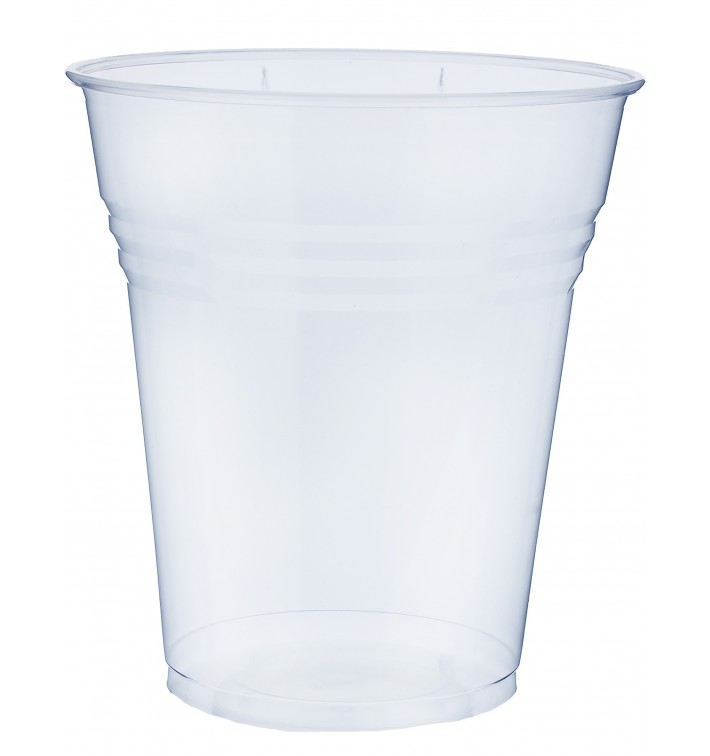
\includegraphics[width = 0.04\textwidth]{Images/transparent_cup.jpg}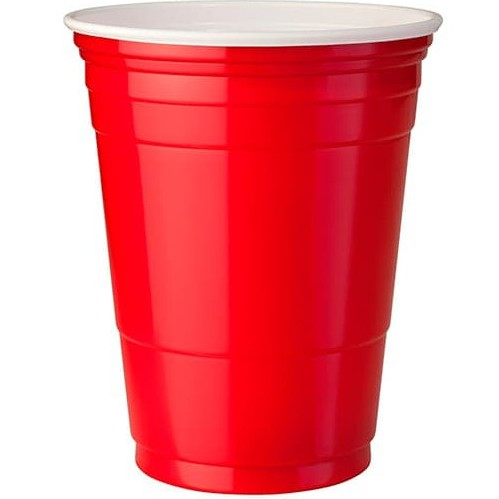
\includegraphics[width = 0.07\textwidth]{Images/red_cup.jpg}};
    \node at (1.5,1.5) {};
    \node at (-1.5,-1.5) {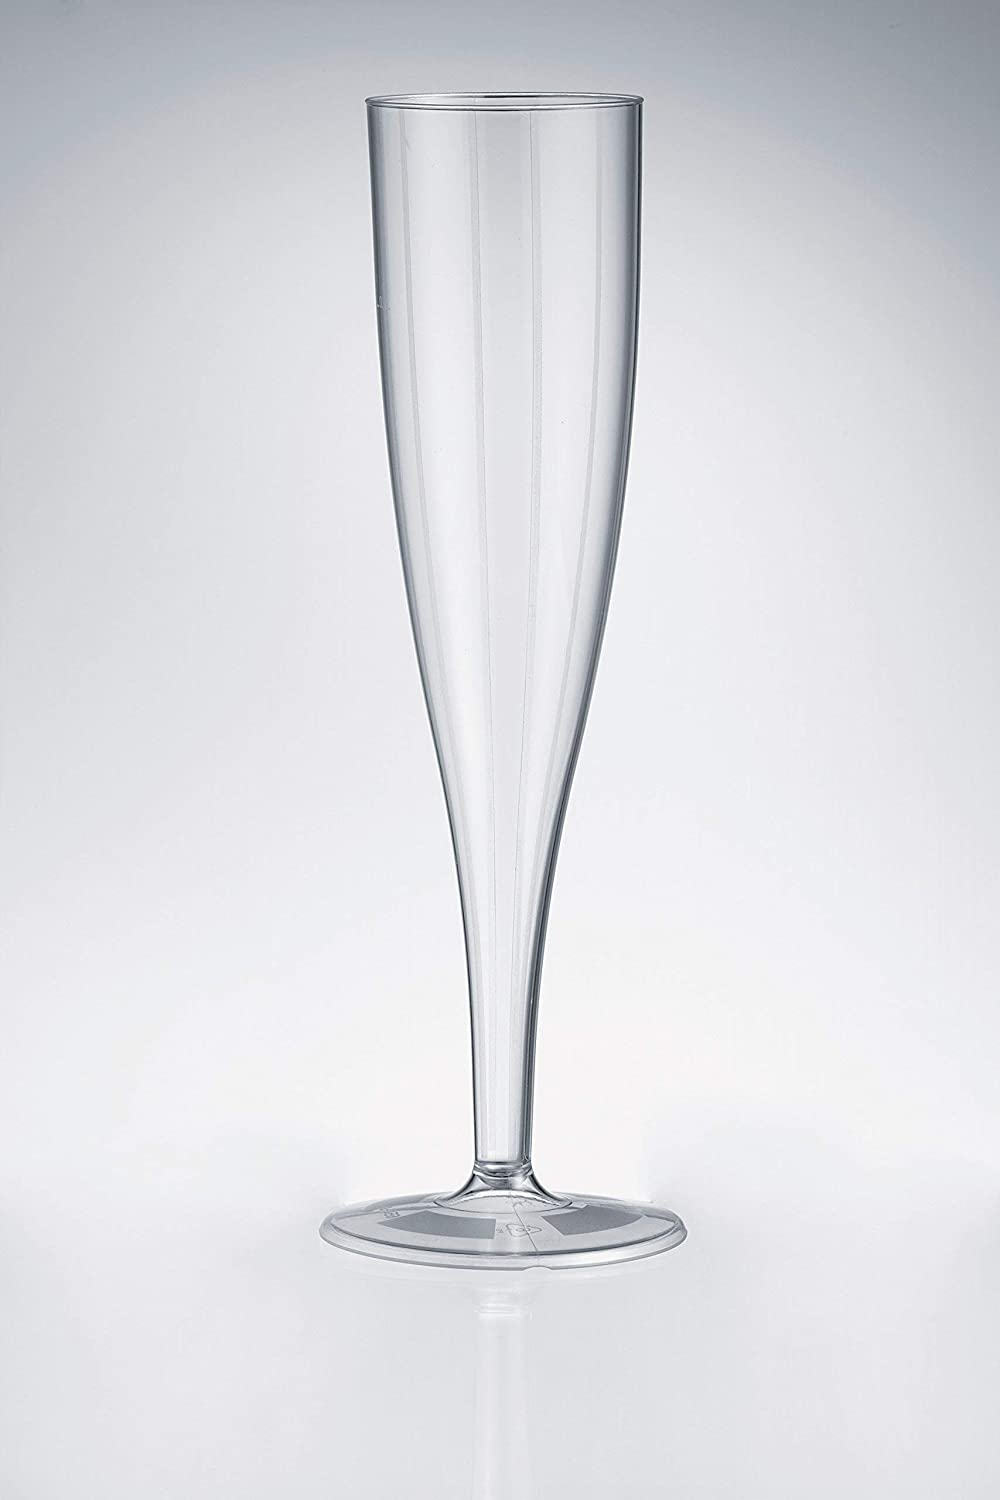
\includegraphics[width = 0.1\textwidth]{Images/champagne_cup.jpg}};
    \node at (1.5,-1.5) {
\includegraphics[width = 0.1\textwidth]{Images/wine_glass1.png}};
  \end{tikzpicture}
  \caption{The two important variables}
  \label{fig:matrix} 
\end{figure}
  
\begin{figure}
  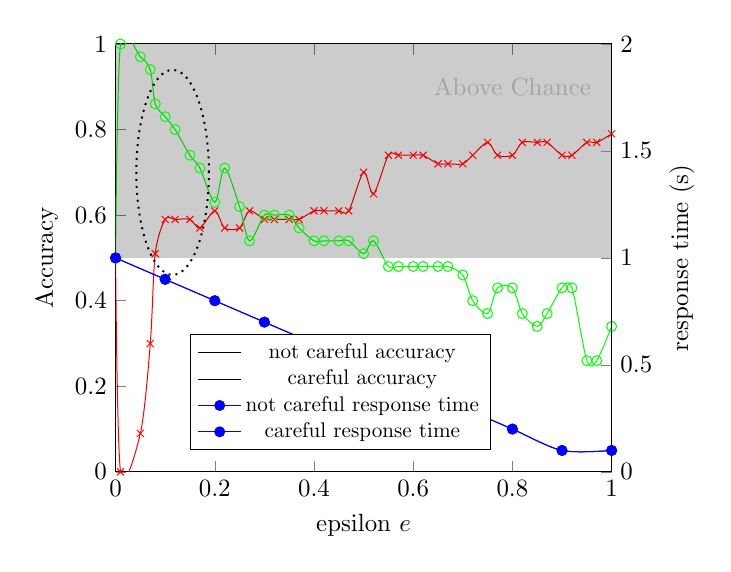
\begin{tikzpicture}[scale=0.9]
\pgfplotsset{
    scale only axis,
    scaled x ticks=base 10:0,
    xmin=0, xmax=1,
    legend style={at={(0.15,0.05)},anchor=south west},
    legend style={nodes={scale=0.85, transform shape}}
}

\begin{axis}[
  axis y line*=left,
  ymin=0, ymax=1,
  xlabel=epsilon $e$,
  ylabel=Accuracy,
]
\addplot[smooth,mark=x,red]
  coordinates{
    (0,0.5)
    (0.01,0)
    (0.05,0.09)
    (0.07,0.3)
    (0.08,0.51)
    (0.1,0.59)
    (0.12,0.59)
    (0.15,0.59)
    (0.17,0.57)
    (0.20,0.61)
    (0.22,0.57)
    (0.25,0.57)
    (0.27,0.61)
    (0.3,0.59)
    (0.32,0.59)
    (0.35,0.59)
    (0.37,0.59)
    (0.4,0.61)
    (0.42,0.61)
    (0.45,0.61)
    (0.47,0.61)
    (0.5,0.70)
    (0.52,0.65)
    (0.55,0.74)
    (0.57,0.74)
    (0.6,0.74)
    (0.62,0.74)
    (0.65,0.72)
    (0.67,0.72)
    (0.70,0.72)
    (0.72,0.74)
    (0.75,0.77)
    (0.77,0.74)
    (0.8,0.74)
    (0.82,0.77)
    (0.85,0.77)
    (0.87,0.77)
    (0.9,0.74)
    (0.92,0.74)
    (0.95,0.77)
    (0.97,0.77)
    (1,0.79)
}; \label{plot_one}

\addplot[smooth,mark=o,green]
  coordinates{
    (0,0.5)
    (0.01,1)
    (0.05,0.97)
    (0.07,0.94)
    (0.08,0.86)
    (0.1,0.83)
    (0.12,0.8)
    (0.15,0.74)
    (0.17,0.71)
    (0.20,0.63)
    (0.22,0.71)
    (0.25,0.62)
    (0.27,0.54)
    (0.3,0.6)
    (0.32,0.6)
    (0.35,0.6)
    (0.37,0.57)
    (0.4,0.54)
    (0.42,0.54)
    (0.45,0.54)
    (0.47,0.54)
    (0.5,0.51)
    (0.52,0.54)
    (0.55,0.48)
    (0.57,0.48)
    (0.6,0.48)
    (0.62,0.48)
    (0.65,0.48)
    (0.67,0.48)
    (0.70,0.46)
    (0.72,0.4)
    (0.75,0.37)
    (0.77,0.43)
    (0.8,0.43)
    (0.82,0.37)
    (0.85,0.34)
    (0.87,0.37)
    (0.9,0.43)
    (0.92,0.43)
    (0.95,0.26)
    (0.97,0.26)
    (1,0.34)
}; \label{plot_two}

% above chance level
\path[top color=black,bottom color=black,middle color=black, fill opacity=0.2] (0,0.5) rectangle (1,1) node[pos=.8] {Above Chance};

% region of interest
\coordinate (a) at (0.1, 0.6);
\coordinate (b) at (0.08,0.85);
\coordinate (c) at (0.15,0.55);
\coordinate (d) at (0.15,0.8);
    \node[ellipse, draw, thick, dotted, 
          fit=(a) (b) (c) (d)] {};
          
\end{axis}

\begin{axis}[
  axis y line*=right,
  axis x line=none,
  ymin=0, ymax=2,
  ylabel=response time (s)
]
\addlegendimage{/pgfplots/refstyle=plot_one}\addlegendentry{not careful accuracy}
\addlegendimage{/pgfplots/refstyle=plot_two}\addlegendentry{careful accuracy}
\addplot[smooth,mark=*,blue]
  coordinates{
    (0,1)
    (0.1,0.9)
    (0.2,0.8)
    (0.3,0.7)
    (0.4,0.6)
    (0.5,0.5)
    (0.6,0.4)
    (0.7,0.3)
    (0.8,0.2)
    (0.9,0.1)
    (1,0.1)
}; \addlegendentry{not careful response time}

\addplot[smooth,mark=*,blue]
  coordinates{
    (0,1)
    (0.1,0.9)
    (0.2,0.8)
    (0.3,0.7)
    (0.4,0.6)
    (0.5,0.5)
    (0.6,0.4)
    (0.7,0.3)
    (0.8,0.2)
    (0.9,0.1)
    (1,0.1)
}; \addlegendentry{careful response time}

\end{axis}

\end{tikzpicture}
  \caption{The evolution of the results for the epsilon}
  \label{fig:class_epsilon}
\end{figure}

\section{Human-Robot Applications}
- for the robot application the model chosen is the most successful model. the one that generalizes best for all people, all cups, and all datasets. 

- you should show a plot with the best model and the rate of change of epsilon. To see how sensitive epsilon is. 
\section{Conclusion}
The conclusion goes here.


% For peer review papers, you can put extra information on the cover
% page as needed:
% \ifCLASSOPTIONpeerreview
% \begin{center} \bfseries EDICS Category: 3-BBND \end{center}
% \fi
%
% For peerreview papers, this IEEEtran command inserts a page break and
% creates the second title. It will be ignored for other modes.
\IEEEpeerreviewmaketitle

% if have a single appendix:
%\appendix[Proof of the Zonklar Equations]
% or
%\appendix  % for no appendix heading
% do not use \section anymore after \appendix, only \section*
% \appendices
% \section{Proof of the First}
% you can choose not to have a title for an appendix
% if you want by leaving the argument blank
% \section{}
% results


% use section* for acknowledgment
\section*{Acknowledgment}

The authors would like to thank...

% Bibliography
\bibliographystyle{ieeetr}
\bibliography{IEEEabrv,references}



\end{document}


